%%%%%%%%%%%%%%%%%%%%%%%%%%%%%%%%%%%%%%%%%%%%%%%%%%%%%%%%%%%%%%%%%
%%%%%%%%%%%%%%%%%%%%%%%%%%%%%%%%%%%%%%%%%%%%%%%%%%%%%%%%%%%%%%%%%
\setcounter{chapter}{4}
\newcommand{\graphicscompanion}{\emph{The \LaTeX{} Graphics Companion}~\cite{graphicscompanion}} 
\newcommand{\hobby}{\emph{A User's Manual for \MP{}}~\cite{metapost}}
\newcommand{\hoenig}{\emph{\TeX{} Unbound}~\cite{unbound}}
\newcommand{\graphicsinlatex}{\emph{Graphics in \LaTeXe{}}~\cite{ursoswald}}

\chapter{Producing Mathematical Graphics}
\label{chap:graphics}

\begin{intro}
Most people use \LaTeX\ for typesetting their text. And since the structure oriented approach to authoring is so convenient, \LaTeX\ also offers a,
if somewhat restricted, means for producing graphical output from textual 
descriptions. Furthermore, quite a number of \LaTeX\ extensions have been created 
in order to overcome these restrictions. In this section, you will learn about a 
few of them.
\end{intro}

\section{Overview}

Creating graphical output with \LaTeX{} has a long tradition. It started out
with the \ei{picture} environment which allows you to create graphics by
cleverly placing predefined elements onto the canvas. A complete
description can be found in the \manual. The \ei{picture} environment of
\LaTeXe\ brings with it the \ci{qbezier} command, ``\texttt{q}'' meaning
``quadratic''.  Many frequently used curves such as circles, ellipses, or
catenaries can be satisfactorily approximated by quadratic B\'ezier curves,
although this may require some mathematical toil. If, in addition, a
programming language is used to generate \ci{qbezier} blocks of \LaTeX\
input files, the \ei{picture} environment becomes quite powerful.

Although programming pictures directly in \LaTeX\ is severely restricted,
and often rather tiresome, there are still reasons for doing so. The documents
thus produced are ``small'' with respect to bytes, and there are no additional
graphics files to be dragged along.

This has been the state of things until a few years ago when Till Tantau of
\pai{beamer} fame came up with the Portable Graphics Format \pai{pgf} and its
companion package TikZ (\pai{tikz}). This system lets you create high
quality vector graphics with all current \TeX{} systems including full
support for pdf.

Building on these basics, numerous packages have been written for specific
purposes. A wide variety of these packages is described in detail in
\graphicscompanion{}.

Perhaps the most advanced graphical tool related with \LaTeX\ is \MP. It is a stand-alone application
based on Donald E. Knuth's \MF. \MP{} has the very powerful and 
mathematically sophisticated programming language of \MF{} but contrary to \MF,
it generates encapsulated \PSi{} files, 
which can be imported in \LaTeX{} and even pdf\LaTeX{}. For an introduction, see \hobby, or the tutorial on \cite{ursoswald}.

A very thorough discussion of \LaTeX{} and \TeX{} strategies for graphics (and fonts) can 
be found in \hoenig.

\section{The \texttt{picture} Environment}
\secby{Urs Oswald}{osurs@bluewin.ch}

As mentioned above the picture environment is part of standard \LaTeX{} and it is great for simple tasks and also if you want
to control the exact positoning of individual elements on a page. But if you are about to do any serious graphics work, you should
look at TikZ as presented in section \ref{sec:tikz} on page \pageref{sec:tikz}.

\subsection{Basic Commands}

A \ei{picture} environment\footnote{Believe it or not, the picture environment works out of the
box, with standard \LaTeXe{} no package loading necessary.} is created with one of the two commands
\begin{lscommand}
\ci{begin}\verb|{picture}(|$x,y$\verb|)|\ldots\ci{end}\verb|{picture}|
\end{lscommand}
\noindent or
\begin{lscommand}
\ci{begin}\verb|{picture}(|$x,y$\verb|)(|$x_0,y_0$\verb|)|\ldots\ci{end}\verb|{picture}|
\end{lscommand}
The numbers $x,\,y,\,x_0,\,y_0$ refer to \ci{unitlength}, which can be reset any time
(but not within a \ei{picture} environment) with a command such as
\begin{lscommand}
\ci{setlength}\verb|{|\ci{unitlength}\verb|}{1.2cm}|
\end{lscommand}
The default value of \ci{unitlength} is \texttt{1pt}. The first pair, $(x,y)$, effects
the reservation, within the document, of rectangular space for the picture. The optional
second pair, $(x_0,y_0)$, assigns arbitrary coordinates to the bottom left corner of the
reserved rectangle. 

Most drawing commands have one of the two forms
\begin{lscommand}
\ci{put}\verb|(|$x,y$\verb|){|\emph{object}\verb|}|
\end{lscommand}
\noindent or
\begin{lscommand}
\ci{multiput}\verb|(|$x,y$\verb|)(|$\Delta x,\Delta y$\verb|){|$n$\verb|}{|\emph{object}\verb|}|\end{lscommand}
B\'ezier curves are an exception. They are drawn with the command
\begin{lscommand}
\ci{qbezier}\verb|(|$x_1,y_1$\verb|)(|$x_2,y_2$\verb|)(|$x_3,y_3$\verb|)|
\end{lscommand}

\subsection{Line Segments}
\begin{example}
\setlength{\unitlength}{5cm}
\begin{picture}(1,1)
  \put(0,0){\line(0,1){1}}
  \put(0,0){\line(1,0){1}}  
  \put(0,0){\line(1,1){1}}  
  \put(0,0){\line(1,2){.5}}
  \put(0,0){\line(1,3){.3333}}
  \put(0,0){\line(1,4){.25}}  
  \put(0,0){\line(1,5){.2}}
  \put(0,0){\line(1,6){.1667}}
  \put(0,0){\line(2,1){1}}
  \put(0,0){\line(2,3){.6667}}
  \put(0,0){\line(2,5){.4}}
  \put(0,0){\line(3,1){1}}  
  \put(0,0){\line(3,2){1}}
  \put(0,0){\line(3,4){.75}}
  \put(0,0){\line(3,5){.6}}
  \put(0,0){\line(4,1){1}}
  \put(0,0){\line(4,3){1}}  
  \put(0,0){\line(4,5){.8}}
  \put(0,0){\line(5,1){1}}
  \put(0,0){\line(5,2){1}}
  \put(0,0){\line(5,3){1}}
  \put(0,0){\line(5,4){1}}
  \put(0,0){\line(5,6){.8333}}
  \put(0,0){\line(6,1){1}}
  \put(0,0){\line(6,5){1}}
\end{picture}
\end{example}
Line segments are drawn with the command
\begin{lscommand}
\ci{put}\verb|(|$x,y$\verb|){|\ci{line}\verb|(|$x_1,y_1$\verb|){|$length$\verb|}}|
\end{lscommand}
The \ci{line} command has two arguments:
\begin{enumerate}
  \item a direction vector,
  \item a length.
\end{enumerate}
The components of the direction vector are restricted to the integers
\[
  -6,\,-5,\,\ldots,\,5,\,6,
\]
and they have to be coprime (no common divisor except 1). The figure illustrates all
25 possible slope values in the first quadrant. The length is relative to \ci{unitlength}.
The length argument is the vertical coordinate in the case of a vertical line segment, the
horizontal coordinate in all other cases.

\subsection{Arrows}

\begin{example}
\setlength{\unitlength}{0.75mm}
\begin{picture}(60,40)
  \put(30,20){\vector(1,0){30}}
  \put(30,20){\vector(4,1){20}}
  \put(30,20){\vector(3,1){25}}
  \put(30,20){\vector(2,1){30}}
  \put(30,20){\vector(1,2){10}}
  \thicklines
  \put(30,20){\vector(-4,1){30}}
  \put(30,20){\vector(-1,4){5}}
  \thinlines
  \put(30,20){\vector(-1,-1){5}}
  \put(30,20){\vector(-1,-4){5}}
\end{picture}
\end{example}
Arrows are drawn with the command
\begin{lscommand}
\ci{put}\verb|(|$x,y$\verb|){|\ci{vector}\verb|(|$x_1,y_1$\verb|){|$length$\verb|}}|
\end{lscommand}
For arrows, the components of the direction vector are even more narrowly restricted than
for line segments, namely to the integers
\[
  -4,\,-3,\,\ldots,\,3,\,4.
\]
Components also have to be coprime (no common divisor except 1). Notice the effect  of the
\ci{thicklines} command on the two arrows pointing to the upper left.

\subsection{Circles}

\begin{example}
\setlength{\unitlength}{1mm}
\begin{picture}(60, 40)
  \put(20,30){\circle{1}}
  \put(20,30){\circle{2}}
  \put(20,30){\circle{4}}
  \put(20,30){\circle{8}}
  \put(20,30){\circle{16}}
  \put(20,30){\circle{32}}
  
  \put(40,30){\circle{1}}
  \put(40,30){\circle{2}}
  \put(40,30){\circle{3}}
  \put(40,30){\circle{4}}
  \put(40,30){\circle{5}}
  \put(40,30){\circle{6}}
  \put(40,30){\circle{7}}
  \put(40,30){\circle{8}}
  \put(40,30){\circle{9}}
  \put(40,30){\circle{10}}
  \put(40,30){\circle{11}}
  \put(40,30){\circle{12}}
  \put(40,30){\circle{13}}
  \put(40,30){\circle{14}}
  
  \put(15,10){\circle*{1}}
  \put(20,10){\circle*{2}}
  \put(25,10){\circle*{3}}
  \put(30,10){\circle*{4}}
  \put(35,10){\circle*{5}}
\end{picture}
\end{example}
The command
\begin{lscommand}
  \ci{put}\verb|(|$x,y$\verb|){|\ci{circle}\verb|{|\emph{diameter}\verb|}}|
\end{lscommand}
\noindent draws a circle with center $(x,y)$ and diameter (not radius) \emph{diameter}.
The \ei{picture} environment only admits diameters up to approximately 14\,mm,
and even below this limit, not all diameters are possible. The \ci{circle*}
command produces disks (filled circles).

As in the case of line segments, one may have to resort to additional packages, 
such as \pai{eepic} or \pai{pstricks}. 
For a thorough description of these packages, see \graphicscompanion.

There is also a possibility within the
\ei{picture} environment. If one is not afraid of doing the necessary calculations
(or leaving them to a program), arbitrary circles and ellipses can be patched
together from quadratic B\'ezier curves. 
See \graphicsinlatex\ for examples and Java source files.

\subsection{Text and Formulas}

\begin{example}
\setlength{\unitlength}{0.8cm}
\begin{picture}(6,5)
  \thicklines
  \put(1,0.5){\line(2,1){3}}
  \put(4,2){\line(-2,1){2}}
  \put(2,3){\line(-2,-5){1}}
  \put(0.7,0.3){$A$}
  \put(4.05,1.9){$B$}
  \put(1.7,2.95){$C$}
  \put(3.1,2.5){$a$}
  \put(1.3,1.7){$b$}
  \put(2.5,1.05){$c$}
  \put(0.3,4){$F=
    \sqrt{s(s-a)(s-b)(s-c)}$}  
  \put(3.5,0.4){$\displaystyle
    s:=\frac{a+b+c}{2}$}
\end{picture}
\end{example}
As this example shows, text and formulas can be written into a \ei{picture} environment with
the \ci{put} command in the usual way.

\subsection{\ci{multiput} and \ci{linethickness}}

\begin{example}
\setlength{\unitlength}{2mm}
\begin{picture}(30,20)
  \linethickness{0.075mm}
  \multiput(0,0)(1,0){26}%
    {\line(0,1){20}}
  \multiput(0,0)(0,1){21}%
    {\line(1,0){25}}
  \linethickness{0.15mm}    
  \multiput(0,0)(5,0){6}%
    {\line(0,1){20}}
  \multiput(0,0)(0,5){5}%
    {\line(1,0){25}}
  \linethickness{0.3mm}    
  \multiput(5,0)(10,0){2}%
    {\line(0,1){20}}
  \multiput(0,5)(0,10){2}%
    {\line(1,0){25}}
\end{picture}
\end{example}
The command
\begin{lscommand}
  \ci{multiput}\verb|(|$x,y$\verb|)(|$\Delta x,\Delta y$\verb|){|$n$\verb|}{|\emph{object}\verb|}|
\end{lscommand}
\noindent has 4 arguments: the starting point, the translation vector from one object to the next, 
the number of objects, and the object to be drawn. The \ci{linethickness} command applies to 
horizontal and vertical line segments, but neither to oblique line segments, nor to circles. 
It does, however, apply to quadratic B\'ezier curves!

\subsection{Ovals}

\begin{example}
\setlength{\unitlength}{0.75cm}
\begin{picture}(6,4)
  \linethickness{0.075mm}
  \multiput(0,0)(1,0){7}%
    {\line(0,1){4}}
  \multiput(0,0)(0,1){5}%
    {\line(1,0){6}}
  \thicklines
  \put(2,3){\oval(3,1.8)} 
  \thinlines
  \put(3,2){\oval(3,1.8)} 
  \thicklines
  \put(2,1){\oval(3,1.8)[tl]} 
  \put(4,1){\oval(3,1.8)[b]} 
  \put(4,3){\oval(3,1.8)[r]} 
  \put(3,1.5){\oval(1.8,0.4)}     
\end{picture}
\end{example}
The command
\begin{lscommand}
  \ci{put}\verb|(|$x,y$\verb|){|\ci{oval}\verb|(|$w,h$\verb|)}|
\end{lscommand}
\noindent or
\begin{lscommand}
  \ci{put}\verb|(|$x,y$\verb|){|\ci{oval}\verb|(|$w,h$\verb|)[|\emph{position}\verb|]}|
\end{lscommand}
\noindent produces an oval centered at $(x,y)$ and having width $w$ and height $h$. The optional 
\emph{position} arguments \texttt{b}, \texttt{t}, \texttt{l}, \texttt{r} refer to 
``top'', ``bottom'', ``left'', ``right'', and can be combined, as the example illustrates. 

Line thickness can be controlled by two kinds of commands: \\ 
\ci{linethickness}\verb|{|\emph{length}\verb|}|
on the one hand, \ci{thinlines} and \ci{thicklines} on the other. While \ci{linethickness}\verb|{|\emph{length}\verb|}|
applies only to horizontal and vertical lines (and quadratic B\'ezier curves), \ci{thinlines} and \ci{thicklines}
apply to oblique line segments as well as to circles and ovals. 


\subsection{Multiple Use of Predefined Picture Boxes}

\begin{example}
\setlength{\unitlength}{0.5mm}
\begin{picture}(120,168)
\newsavebox{\foldera}
\savebox{\foldera}
  (40,32)[bl]{% definition 
  \multiput(0,0)(0,28){2}
    {\line(1,0){40}}
  \multiput(0,0)(40,0){2}
    {\line(0,1){28}}
  \put(1,28){\oval(2,2)[tl]}
  \put(1,29){\line(1,0){5}}
  \put(9,29){\oval(6,6)[tl]}
  \put(9,32){\line(1,0){8}}
  \put(17,29){\oval(6,6)[tr]}
  \put(20,29){\line(1,0){19}}
  \put(39,28){\oval(2,2)[tr]}  
}
\newsavebox{\folderb}
\savebox{\folderb}
  (40,32)[l]{%         definition 
  \put(0,14){\line(1,0){8}}
  \put(8,0){\usebox{\foldera}}
}
\put(34,26){\line(0,1){102}} 
\put(14,128){\usebox{\foldera}}
\multiput(34,86)(0,-37){3}
  {\usebox{\folderb}} 
\end{picture}
\end{example}
A picture box can be \emph{declared} by the command
\begin{lscommand}
  \ci{newsavebox}\verb|{|\emph{name}\verb|}|
\end{lscommand}
\noindent then \emph{defined} by  
\begin{lscommand}
  \ci{savebox}\verb|{|\emph{name}\verb|}(|\emph{width,height}\verb|)[|\emph{position}\verb|]{|\emph{content}\verb|}|
\end{lscommand}
\noindent and finally arbitrarily often be \emph{drawn} by
\begin{lscommand}
  \ci{put}\verb|(|$x,y$\verb|){|\ci{usebox}\verb|{|\emph{name}\verb|}}|
\end{lscommand}

The optional \emph{position} parameter has the effect of defining the
`anchor point' of the savebox. In the example it is set to \texttt{bl} which
puts the anchor point into the bottom left corner of the savebox. The other
position specifiers are \texttt{t}op and \texttt{r}ight.

The \emph{name} argument refers to a \LaTeX{} storage bin and therefore is
of a command nature (which accounts for the backslashes in the current
example). Boxed pictures can be nested: In this example, \ci{foldera} is
used within the definition of \ci{folderb}.

The \ci{oval} command had to be used as the \ci{line} command does not work if the segment length is less than 
about 3\,mm.

\subsection{Quadratic B\'ezier Curves}

\begin{example}
\setlength{\unitlength}{0.8cm}
\begin{picture}(6,4)
  \linethickness{0.075mm}
  \multiput(0,0)(1,0){7}
    {\line(0,1){4}}
  \multiput(0,0)(0,1){5}
    {\line(1,0){6}}
  \thicklines
  \put(0.5,0.5){\line(1,5){0.5}}    
  \put(1,3){\line(4,1){2}} 
  \qbezier(0.5,0.5)(1,3)(3,3.5)
  \thinlines   
  \put(2.5,2){\line(2,-1){3}}
  \put(5.5,0.5){\line(-1,5){0.5}}
  \linethickness{1mm}
  \qbezier(2.5,2)(5.5,0.5)(5,3)
  \thinlines
  \qbezier(4,2)(4,3)(3,3)
  \qbezier(3,3)(2,3)(2,2)
  \qbezier(2,2)(2,1)(3,1)
  \qbezier(3,1)(4,1)(4,2)
\end{picture}
\end{example}
As this example illustrates, splitting up a circle into 4 quadratic B\'ezier curves
is not satisfactory. At least 8 are needed. The figure again shows the effect of
the \ci{linethickness} command on horizontal or vertical lines, and of the 
\ci{thinlines} and the \ci{thicklines} commands on oblique line segments. It also 
shows that both kinds of commands affect quadratic B\'ezier curves, each command
overriding all previous ones.

Let $P_1=(x_1,\,y_1),\,P_2=(x_2,\,y_2)$ denote the end points, and $m_1,\,m_2$ the
respective slopes, of a quadratic B\'ezier curve. The intermediate control point 
$S=(x,\,y)$ is then given by the equations
\begin{equation} \label{zwischenpunkt}
  \left\{
    \begin{aligned}{rcl}
      x & = & \displaystyle \frac{m_2 x_2-m_1x_1-(y_2-y_1)}{m_2-m_1}, \\
      y & = & y_i+m_i(x-x_i)\qquad (i=1,\,2).
    \end{aligned}
  \right.
\end{equation}
\noindent See \graphicsinlatex\ for a Java program which generates
the necessary \ci{qbezier} command line.

\subsection{Catenary}

\begin{example}
\setlength{\unitlength}{1cm}
\begin{picture}(4.3,3.6)(-2.5,-0.25)
\put(-2,0){\vector(1,0){4.4}}
\put(2.45,-.05){$x$}
\put(0,0){\vector(0,1){3.2}}
\put(0,3.35){\makebox(0,0){$y$}}
\qbezier(0.0,0.0)(1.2384,0.0)
  (2.0,2.7622) 
\qbezier(0.0,0.0)(-1.2384,0.0)
  (-2.0,2.7622)
\linethickness{.075mm}
\multiput(-2,0)(1,0){5}
  {\line(0,1){3}}
\multiput(-2,0)(0,1){4}
  {\line(1,0){4}}
\linethickness{.2mm}
\put( .3,.12763){\line(1,0){.4}}
\put(.5,-.07237){\line(0,1){.4}}
\put(-.7,.12763){\line(1,0){.4}}
\put(-.5,-.07237){\line(0,1){.4}}
\put(.8,.54308){\line(1,0){.4}}
\put(1,.34308){\line(0,1){.4}}
\put(-1.2,.54308){\line(1,0){.4}}
\put(-1,.34308){\line(0,1){.4}}
\put(1.3,1.35241){\line(1,0){.4}}
\put(1.5,1.15241){\line(0,1){.4}}
\put(-1.7,1.35241){\line(1,0){.4}}
\put(-1.5,1.15241){\line(0,1){.4}}
\put(-2.5,-0.25){\circle*{0.2}}
\end{picture}
\end{example}

In this figure, each symmetric half of the catenary $y=\cosh x -1$ is approximated by a quadratic
B\'ezier curve. The right half of the curve ends in the point \((2,\,2.7622)\), the slope there having the value 
\(m=3.6269\). Using again equation (\ref{zwischenpunkt}), we can 
calculate the intermediate control points. They turn out to be $(1.2384,\,0)$ and $(-1.2384,\,0)$. 
The crosses indicate points of the \emph{real} catenary. The error is barely noticeable, being less 
than one percent.

This example points out the use of the optional argument of the \\
\verb|\begin{picture}| command.
The picture is defined in convenient ``mathematical'' coordinates, whereas by the command
\begin{lscommand} 
  \ci{begin}\verb|{picture}(4.3,3.6)(-2.5,-0.25)|
\end{lscommand}
\noindent its lower left corner (marked by the black disk) is assigned the coordinates $(-2.5,-0.25)$. 

\subsection{Rapidity in the Special Theory of Relativity}

\begin{example}
\setlength{\unitlength}{0.8cm}
\begin{picture}(6,4)(-3,-2)
  \put(-2.5,0){\vector(1,0){5}}
  \put(2.7,-0.1){$\chi$}
  \put(0,-1.5){\vector(0,1){3}}
  \multiput(-2.5,1)(0.4,0){13}
    {\line(1,0){0.2}}
  \multiput(-2.5,-1)(0.4,0){13}
    {\line(1,0){0.2}}
  \put(0.2,1.4)
    {$\beta=v/c=\tanh\chi$}
  \qbezier(0,0)(0.8853,0.8853)
    (2,0.9640)
  \qbezier(0,0)(-0.8853,-0.8853)
    (-2,-0.9640)
  \put(-3,-2){\circle*{0.2}}
\end{picture}
\end{example}
The control points of the two B\'ezier curves were calculated with formulas (\ref{zwischenpunkt}).
The positive branch is determined by $P_1=(0,\,0),\,m_1=1$ and $P_2=(2,\,\tanh 2),\,m_2=1/\cosh^2 2$.
Again, the picture is defined in mathematically convenient coordinates, and the lower left corner
is assigned the mathematical coordinates $(-3,-2)$ (black disk).

\section{The PGF and TikZ Graphics Packages}
\label{sec:tikz}

Today every \LaTeX{} output generation system can create nice vector graphics,
it's just the interfaces that are rather diverse. The \pai{pgf} package provides an
abstraction layer over these interface. The
\pai{pgf} package comes with a large manual/tutorial of its own
\cite{pgfplot}. So we are only going to scratch the surface of the package with this little
section.

The \pai{pgf} package comes with a high level access language provided by the  \pai{tikz} package.
TikZ provides highly efficient commands to
draw graphics right from inside your document. Use the \ei{tikzpicture}
environment to wrap your TikZ commands.

As mentioned above, there is an excellent manual for \pai{pgf} and friends. So
instead of actually explaining how it works, I will just show you a few examples
so that you can get a first impression of how this tool works.

First a simple nonsense diagram.
\begin{example}
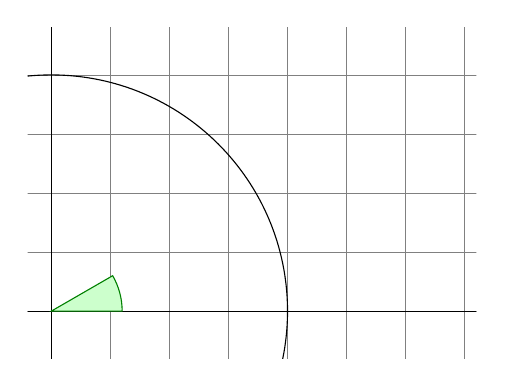
\begin{tikzpicture}[scale=3]
  \clip (-0.1,-0.2)
     rectangle (1.8,1.2);
  \draw[step=.25cm,gray,very thin]
       (-1.4,-1.4) grid (3.4,3.4);
  \draw (-1.5,0) -- (2.5,0);
  \draw (0,-1.5) -- (0,1.5);
  \draw (0,0) circle (1cm);
  \filldraw[fill=green!20!white,
            draw=green!50!black]
    (0,0) -- (3mm,0mm) 
         arc (0:30:3mm) -- cycle;
\end{tikzpicture}
\end{example}
Note the semicolon (\texttt{;}) character. It separates the individual commands.

A simple Venn diagram.
\begin{example}
\shorthandoff{:}
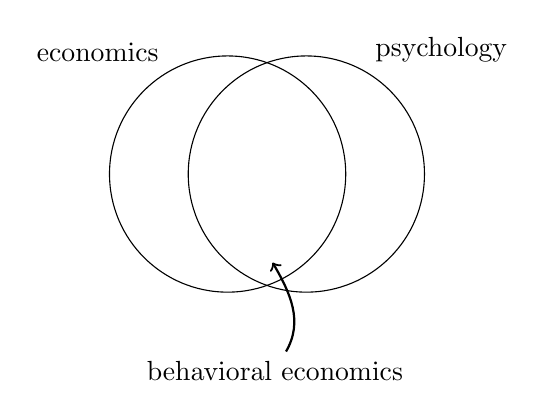
\begin{tikzpicture}
  \node[circle,draw,
        minimum size=3cm,
        label=120:{economics}]
         at (0,0) {};
  \node[circle,draw,
        minimum size=3cm,
        label=60:{psychology}]
         at (1,0) {};
  \node (i) at (0.5,-1) {};
  \node at (0.6,-2.5) 
    {behavioral economics}
    edge[->,thick,
         out=60,in=-60] (i);
\end{tikzpicture}
\end{example}
If you are using \pai{tikz} in connection with \pai{babel} some of the characters used in the
TikZ language may get modified by \pai{babel}, leading to odd errors. To counteract this, add 
the \ci{shorthandoff} command to your code.

Note the foreach loops in the next example.
\begin{example}
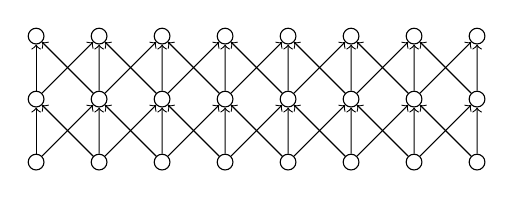
\begin{tikzpicture}[scale=0.8]
  \tikzstyle{v}=[circle, minimum size=2mm,inner sep=0pt,draw]
  \foreach \i in {1,...,8}
    \foreach \j in {1,...,3}
      \node[v] 
        (G-\i-\j) at (\i,\j) {};
  \foreach \i in {1,...,8}
    \foreach \j/\o in {1/2,2/3}
      \draw[->] 
        (G-\i-\j) -- (G-\i-\o);
  \foreach \i/\n in 
    {1/2,2/3,3/4,4/5,5/6,6/7,7/8}
    \foreach \j/\o in {1/2,2/3} {
       \draw[->] (G-\i-\j) -- (G-\n-\o);
       \draw[->] (G-\n-\j) -- (G-\i-\o);
    }
\end{tikzpicture}
\end{example}

With the \ci{usetikzlibrary}
command in the preamble you can enable a wide variety of additional
features for drawing special shapes, like this box which is slightly bent.
\begin{example}
\usetikzlibrary{%
  decorations.pathmorphing}
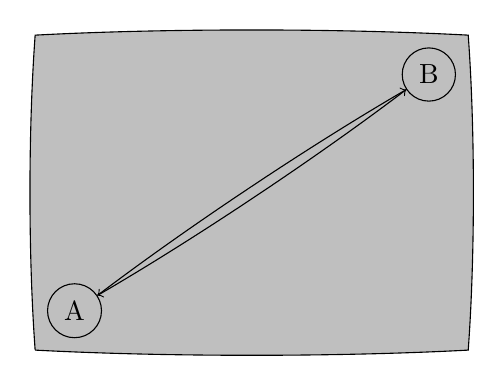
\begin{tikzpicture}[
     decoration={bent,aspect=.3}]
 \draw [decorate,fill=lightgray]
        (0,0) rectangle (5.5,4);
 \node[circle,draw] 
        (A) at (.5,.5) {A};
 \node[circle,draw] 
        (B) at (5,3.5) {B};
 \draw[->,decorate] (A) -- (B);
 \draw[->,decorate] (B) -- (A);
\end{tikzpicture}
\end{example}

\begin{example}
\usetikzlibrary{positioning}
\begin{tikzpicture}[xscale=6,
     yscale=8,>=stealth]
  \tikzstyle{v}=[circle,
     minimum size=1mm,draw,thick]
  \node[v] (a) {$1$};
  \node[v] (b) [right=of a] {$2$};
  \node[v] (c) [below=of a] {$2$};
  \node[v] (d) [below=of b] {$1$};
  \draw[thick,->] 
        (a) to node {} (c);
  \draw[thick,->] 
        (a) to node {} (d);
  \draw[thick,->] 
        (b) to node {} (d);
\end{tikzpicture}
\end{example}

You can even draw syntax diagrams that look as if they came straight from a book on
Pascal programming. The code is a bit more daunting than the example above,
so I will just show you the result. If you have a look at the \pai{pgf} documentation
you will find a detailed tutorial on drawing this exact diagram.

\begin{center}
\begin{tikzpicture}[point/.style={coordinate},thick,draw=black!50,>=stealth',
                    tip/.style={->,shorten >=1pt},every join/.style={rounded corners},
                    skip loop/.style={to path={-- ++(0,#1) -| (\tikztotarget)}},
                    hv path/.style={to path={-| (\tikztotarget)}},
                    vh path/.style={to path={|- (\tikztotarget)}},
                 terminal/.style={
            rounded rectangle,
            minimum size=6mm,
            thick,draw=black!50,
            top color=white,bottom color=black!20,
            font=\ttfamily\tiny},
                nonterminal/.style={
                       rectangle,
                       minimum size=6mm,
                       thick,
                       draw=red!50!black!50,         % 50% red and 50% black,
                       top color=white,              % a shading that is white at the top...
                       bottom color=red!50!black!20, % and something else at the bottom
                       font=\itshape\tiny}]
\matrix[column sep=4mm] {
  % First row:
  & & & & & & & & & & & \node (plus) [terminal] {+};\\
  % Second row:
  \node (p1) [point] {}; &     \node (ui1)    [nonterminal] {unsigned integer}; &
  \node (p2) [point] {}; &     \node (dot)    [terminal]    {.};                &
  \node (p3) [point] {}; &     \node (digit) [terminal]     {digit};            &
  \node (p4) [point] {}; &     \node (p5)     [point] {};                       &
  \node (p6) [point] {}; &     \node (e)      [terminal]    {E};                &
  \node (p7) [point] {}; &                                                      &
  \node (p8) [point] {}; &     \node (ui2)    [nonterminal] {unsigned integer}; &
  \node (p9) [point] {}; &     \node (p10)    [point]       {};\\
  % Third row:
  & & & & & & & & & & & \node (minus)[terminal] {-};\\
};
{ [start chain]
  \chainin (p1);
  \chainin (ui1)   [join=by tip];
  \chainin (p2)    [join];
  \chainin (dot)   [join=by tip];
  \chainin (p3)    [join];
  \chainin (digit) [join=by tip];
  \chainin (p4)    [join];
  { [start branch=digit loop]
    \chainin (p3) [join=by {skip loop=-6mm,tip}];
  }
  \chainin (p5)    [join,join=with p2 by {skip loop=6mm,tip}];
  \chainin (p6)    [join];
  \chainin (e)     [join=by tip];
  \chainin (p7)    [join];
  { [start branch=plus]
    \chainin (plus) [join=by {vh path,tip}];
    \chainin (p8)    [join=by {hv path,tip}];
  }
  { [start branch=minus]
    \chainin (minus) [join=by {vh path,tip}];
    \chainin (p8)    [join=by {hv path,tip}];
  }
  \chainin (p8)    [join];
  \chainin (ui2)   [join=by tip];
  \chainin (p9)    [join,join=with p6 by {skip loop=-11mm,tip}];
  \chainin (p10)   [join=by tip];
}
\end{tikzpicture}
\end{center}

And there is more, if you have to draw plots of numerical data or
functions, you should have a closer look at the  \pai{pgfplot}
package. It provides everything you need to draw plots. It can even
call the external \texttt{gnuplot} command to evaluate actual
functions you wrote into the graph.

For more inspiration make sure to visit Kjell Magne Fauske's excellent
\url{http://www.texample.net/tikz/}. it contains an ever expanding store of
beautiful graphs and other \LaTeX{} code. On \TeX{}ample.net you will also
find a
 \href{http://www.texample.net/tikz/resources/#tools-that-generate-pgftikz-code}{list
 of tools to work with PGF/TikZ} so that you do not have to write all that
 code by hand.

%%% Local Variables:
%%% TeX-master: "lshort.tex"
%%% mode: flyspell
%%% TeX-PDF-mode: t
%%% End:
